\subsection{Features Extraction}
\label{subsec:features}

Feature extraction is performed using \textit{Chroma Toolbox} \cite{ChromaToolbox}, a MATLAB implementation of many different features under GPL license.\\
%
At first, the audio signal is decomposed into 88 frequency bands centered in the frequencies corresponding to the pitches of A0 up to C8. A multirate filter bank using elliptic filters is used and finally \textit{Short-Time Mean-Square Power} (STMSP) is used to extract the useful information. In order to ignore the the different harmonicities given by different instruments, the energies referred to the same notes are pooled together resulting in 12-dimensional vectors.\\
%
The different features are then obtained operating in different ways on the extracted pitches. In this project we used three of them:
\begin{itemize}
	\item CLP (\textit{Chroma Features with Logarithmic Compression}): bands from different octaves are summed together, a logarithmic function is applied (to emulate our logarithmic perception of sound intensity) and then the vector is normalized to $L_2$-norm equal to 1.
	\item CENS (\textit{Chroma Energy Normalized Statistics}): in order to account for dynamics, timbre, articulation, execution of note groups, and temporal micro-deviations, smart logarithmic quantization, temporal smoothing, downsampling and normalizations are performed.
	\item CRP (\textit{Chroma DCT-Reduced log Pitch}): they include logarithmic compression, smoothing and timbre invariance by using a DCT-based technique.
\end{itemize}

\begin{figure*}[t]
	\hfill
	\begin{subfigure}[b]{.45\linewidth}
		\centering
		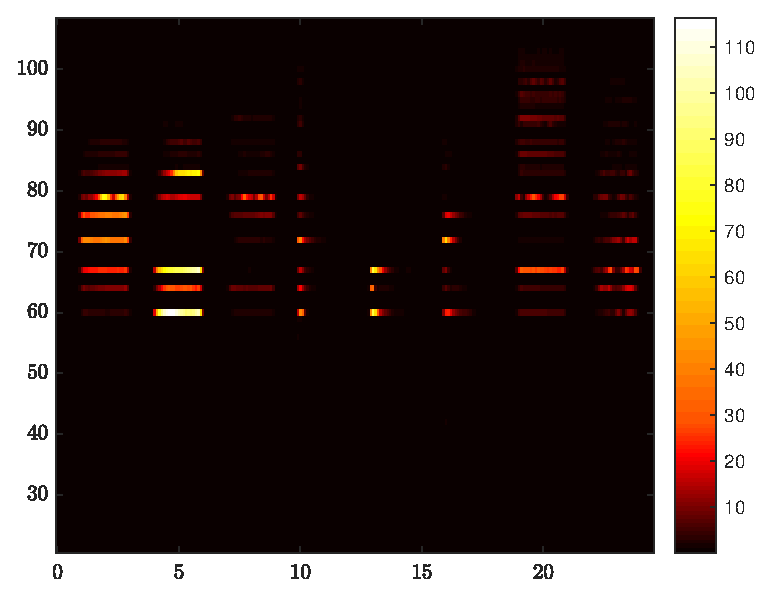
\includegraphics[width=0.7\linewidth]{img/PitchExample}
		\caption{Example of pitch extraction}
		\label{fig:PitchExample}
	\end{subfigure}
	\hfill
	\begin{subfigure}[b]{.45\linewidth}
		\centering
		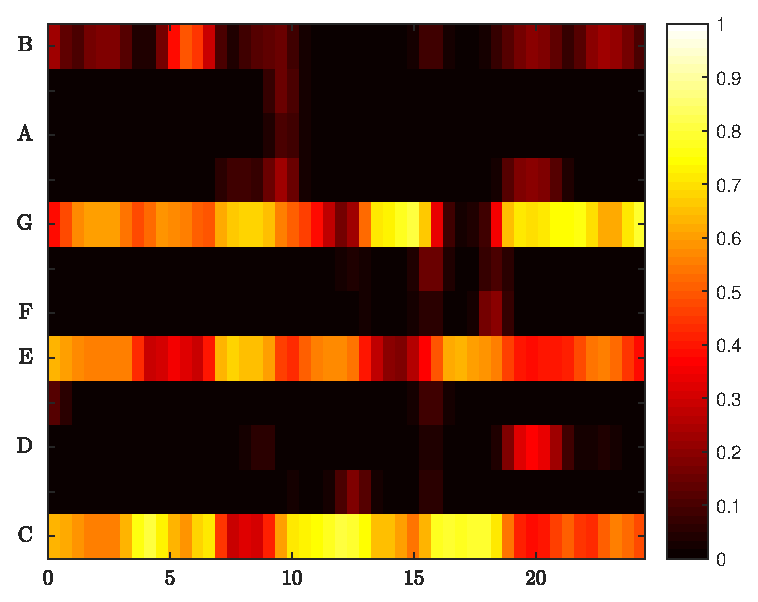
\includegraphics[width=0.7\linewidth]{img/CENSexample}
		\caption{Example of CENS features}
		\label{fig:CENSexample}
	\end{subfigure}
	\hfill
\end{figure*}
